\documentclass[../monografia.tex]{subfiles}
\graphicspath{ {images/}{../images/}{../../images/} }

\begin{document}

\chapter{Conceptual Aspects}
\label{chapter: Conceptual Aspects}

Dealing with a complete simulation of an embedded system there are three main problems: microcontroller emulation, environment simulation and the interconnection between both.

\textbf{Microcontroller Emulation}: The main aspects of the microcontroller must be emulated, including: microprocessing, General Purpose Input Output, RAM memory, flash memory  and others peripherals present in the device.

\textbf{Environment Simulation}: The embedded device is always immersed in an environment, therefore it's simulation must be able to replicate a variety of natural physical phenomena, in addition to being easily manipulated and adaptable.

\textbf{Integration}: The integration between them should capture the phenomena obtained from the environment simulation and send the data to the microcontroller emulator as if they were electrical signals it would receive in reality. Conversely, the integration must also capture the values calculated by the emulation and send them back to the virtual environment. This cycle should occur continuously.

%---
\begin{figure}[h!]
    \caption{General concept}
    \centering % para centralizarmos a figura
    \includegraphics[width=14cm]{General concept.png}
    \label{fig: General concept}
\end{figure}
%---

In this undergraduate final project, those three main problems will be addressed. To achieve this, industry-standard tools will be used to implement microcontroller emulation, environment simulation, and design. Additionally, there is currently no available tool capable of effectively connecting these features.

% ----------------------------------------------------------
% MICROCONTROLLER
% ----------------------------------------------------------
\section{Microcontroller Emulation}

Embedded devices are designed primarily to execute specific functions or to address particular applications, with inherent data processing capabilities. Microcontrollers are widely used to achieve this goal. However, it’s important to have a clear understanding of their concepts and functioning due to the complexity and diversity of these chips.

\subsection{What is a Microcontroller}

A microcontroller is a programmable embedded electronic device that integrates a processor, memory, and peripherals into a single integrated circuit. These devices have specific architectures that vary depending on the manufacturer and include a range of peripherals designed to perform specific functions.

Microcontrollers typically feature 8-bit, 16-bit, or 32-bit architectures. Each architecture organizes information in memory differently, which affects aspects such as storage capacity and address management, among other factors.

The microcontroller's peripherals are responsible for communication with external environment. They play a role in receiving sensor information, managing communication interfaces, and sending signals, which translates into actions in the external world.

Initially, the peripherals receive and send a series of electrical signals originating from various sensors and actuators, which access the internal circuits of the microcontroller. These signals modify the microcontroller’s memory. When the microcontroller reads the information stored in memory, it detects any changes and, if needed, adjusts its output behavior accordingly.
%---
\begin{figure}[h!]
\centering
    \caption{Microcontroller basic structure}
    \centering % para centralizarmos a figura
    \includegraphics[width=14cm]{microcontroller_structure.png}
    \par
    Source: ElectronicsHub \cite{eletronic_hub_23}
    \label{fig: Microcontroller basic structure}
\end{figure}
%---

In the context of simulation, it is essential to replicate these external world functionalities, which are the responsibilities of the peripherals. Due to the specific way each peripheral accesses reserved positions in the microcontroller's memory and organizes information, it is important to explain in greater detail how this process is carried out for the peripherals that are the focus of emulation in this project.

\subsubsection{General Purpose Input/Output (GPIO)}

The GPIOs (General Purpose Input/Output) are fundamental peripherals in microcontrollers, responsible for handling information in a binary form, represented as 0 or 1. In the context of microcontrollers, it is necessary to specify which PORT and PIN will be used to configure a particular GPIO. This selection ensures that the appropriate pin is allocated within the circuit in which the microcontroller is integrated.

GPIOs function as MMOI (Memory Mapped Input/Output), which means they map a specific memory location to store information related to the PORT and PIN. Each port corresponds to a specific memory address, while each pin acts as a mask that indicates the memory position where the information is being stored.


%---
\begin{figure}[h]
\centering
    \caption{GPIO addresses from microcontroller STM32F103C8T6}
    \centering % para centralizarmos a figura
    \includegraphics[width=14cm]{GPIO_addresses.png}
    \par
    Fonte: STM32F103C8T6 Datasheet \cite{STM32F103C8T6_Datasheet_23}
    \label{fig: GPIO addresses from microcontroller STM32F103C8T6}
\end{figure}
%---

Additionally, the GPIO configuration—such as whether it will be used as an input or output or for other functions—also influences the memory location that will be accessed to retrieve the necessary information.


% ----------------------------------------------------------
% ENVIRONMENT
% ----------------------------------------------------------
\section{Environment Simulation}
\subsection{Modeling the environment}
The scope of modeling refers to how the simulation will be visualized. The two main objects that need to be modeled are the room and the embedded system itself. To achieve this, there is a variety of open-source software that provides modeling tools and can export the created objects to the simulation environment.

\subsection{Running the environment}
The running environment integrates the modeled objects, including all their physical characteristics and interactions. It will also be responsible for exporting and receiving data to and from an external source.

% ----------------------------------------------------------
% INTEGRATION
% ----------------------------------------------------------
\section{Integration between the simulation and the emulation}
Nowadays there are many ways to make the interconnection and data exchange between between two different software.

For this project, it is necessary  a non-stop data exchange of both sides between the emulation and the simulation. To accomplish that, it is interesting to use used communication protocols that is shown as it follows:

\subsection{Protocol Buffers}
Protocol buffers \cite{google_protocol_buffers}, or protobufs, are mechanism developed by Google used to serialize different kind of data. Using a  language and platform neutral schema definition, protobufs are really useful to parse and serialize data between software that uses different types of languages and formats.

To define how the data is structured, it is used the \texttt{.proto} files. These files needs to be compiled by the proto compiler to generate the source code structuring the data format in different types of languages. In that way, the same \texttt{.proto} file can used by different software.

%---
\begin{figure}[h]
\centering
    \caption{Protocol Buffer workflow}
    \centering % para centralizarmos a figura
    \includegraphics[width=14cm]{protobuf_workflow.png}
    \label{fig: protobuf_workflow}
\end{figure}
%---

An important feature of this protocol is how its messages are compact. Using a compact binary format reduces the network load on the application.

\subsection{Publishers and Subscribers}
This messaging pattern \cite{publisher_subscriber} is used to facilitate communication between different parts of a system or different software components. This pattern is based on what is known as a "topic," which acts as a channel that allows two possible actions: publishing and subscribing.

%---
\begin{figure}[h]
\centering
    \caption{Publisher-Subscriber Pattern}
    \centering % para centralizarmos a figura
    \includegraphics[width=14cm]{publish-subscribe.png}
    \label{fig: publisher subscriber pattern}
\end{figure}
%---

Publishing means sending a message to a topic, making that message visible to anyone with reading access to the topic. It allows data to be shared via the topic.

On the other hand, subscribing means ‘listening’ to what is published on a topic. When a topic is published, the subscriber receives a callback notifying them of the message’s arrival and retrieving the data.

% ----------------------------------------------------------
% KVN AND EMULATION
% ----------------------------------------------------------
\section{Kernel Virtual Machine and Emulation}

\subsection{Kernel Virtual Machine}

%---
\begin{wrapfigure}{r}{7cm}
    \centering
    \caption{KVM Architecture}
    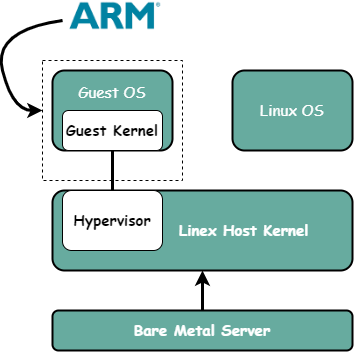
\includegraphics[width=7cm]{diagramas-concentual_aspects_kvm.drawio.png}
    \label{fig: KVM Architecture}
\end{wrapfigure}
%---

System virtualization is the process of hosting one operating system (the guest system) within another (the host system). Through virtualization, the guest system can replicate its functionalities by leveraging the host system's processing power. This allows the host to run functionalities exclusive to the guest system.

Virtualization is made possible by the use of a hypervisor, a type of operating system-level software responsible for managing the host system's computing resources and allocating them to hosted virtual machines.

In this context, the Kernel Virtual Machine (KVM) \cite{Linux_KVM_23} is a technology used for virtualization on Linux systems. It transforms the Linux kernel into a hypervisor, enabling part of the host hardware to be directly utilized for guest system functionalities. For instance, KVM maps the virtualized guest memory directly to the host memory and allows the host processor to function as a virtualized CPU.

This approach enables the guest system to run nearly as if it were native, significantly improving performance, security, and reliability.

For our project, KVM is particularly useful for emulating all the specific components of a microcontroller (such as an ARM microcontroller \cite{wikipedia_arm_architecture_24}), including the processor, memory, peripherals, and more.

% - explicar que KVM é um virtualizador
% - divide parte da CPU do sistema host com o guest
% - sua atuação ajuda a sistemas emulados possuírem performances perto da nativa, devido a virtualização direta no host

\subsection{Emulation}

In computing, emulation refers to the process of replicating the behavior of one computer system or software on another system.

In this context, hardware emulation involves replicating the functionalities of hardware components such as memory management, I/O operations, CPU processing, and interrupt handling within another system. Unlike simulation, which models how a system behaves in theory, emulation strives to replicate the original system's actual operation. This enables the emulated system to use the same configurations, load identical software, and adhere to the same standards as the original hardware.

An ideal hardware emulation accurately reproduces every functionality of the original system, maintaining full compatibility.

% - Explicar o que é emulação
% - O que é emular um hardware

% ----------------------------------------------------------
% PIONER 2DX and P2OS
% ----------------------------------------------------------
\section{Real Robot hardware and communication}

\subsection{Pioneer 2DX}

%---
\begin{wrapfigure}{r}{6cm}
    \centering
    \caption{Pioneer 2}
    \includegraphics[width=6cm]{pioneer2.png}
    \label{fig: Pioneer 2}
\end{wrapfigure}
%---

The Pioneer 2 is a programmable mobile robot platform widely used in research and educational settings for the development and testing of robotics algorithms and systems worldwide. The Pioneer 2 supports a variety of sensors and actuators, such as motors, ultrasonic sensors, encoders, cameras, and more. This enables it to perform tasks like navigation, mapping, and object manipulation in diverse environments.

Designed for research and education, the Pioneer 2 serves as a tool for exploring conceptual aspects of robotics, including kinematics, path planning, and sensor fusion.

As a commercial robot, there is an operations manual available for users \cite{pioneer2dx_2024}, which includes all hardware specifications and detailed instructions on how to use the robot correctly.

\subsubsection{Communication}

For communication with the robot, there is a Serial RS232 port available. The pins for this serial port are listed in Table \ref{table: P2OS Internal Serial Port Connections ("HOST" JP8)}. The TX and RX pins allow external devices to communicate with the Pioneer 2DX through the P2OS protocol, which is further described in Section \ref{P2OS - Communication protocol}.


\begin{table}[h!]
\centering
\caption{P2OS Internal Serial Port Connections ("HOST" JP8)}
\label{table: P2OS Internal Serial Port Connections ("HOST" JP8)}
\begin{tabular}{|c|l|l|c|l|}
\cline{1-2} \cline{4-5}
\textbf{Pin \#} & \textbf{Connection} &  & \textbf{Pin \#} & \textbf{Connection} \\ \cline{1-2} \cline{4-5} 
1               & Gnd                 &  & 2               & P3\_12              \\ \cline{1-2} \cline{4-5} 
3               & TxD1                &  & 4               & 12 VDC (switched)   \\ \cline{1-2} \cline{4-5} 
5               & RxD1                &  & 6               & Gnd                 \\ \cline{1-2} \cline{4-5} 
7               & P3\_15              &  & 8               & P3\_14              \\ \cline{1-2} \cline{4-5} 
9               & Gnd                 &  & 10              & 5 VDC (switched)    \\ \cline{1-2} \cline{4-5} 
\end{tabular}

\vspace{2mm}

Source: Pioneer2 Operations Manual \cite{pioneer2dx_2024}
\end{table}

\clearpage

\section{P2OS - Communication protocol}
\label{P2OS - Communication protocol}
%---
\begin{wrapfigure}{r}{6cm}
    \centering
    \caption{P2OS Connection}
    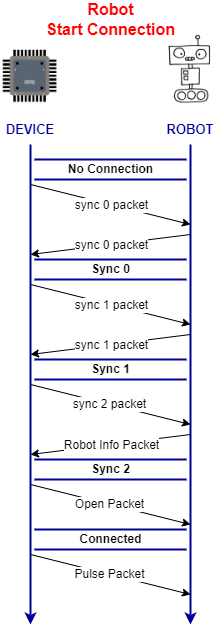
\includegraphics[width=6cm]{diagramas-p2os.drawio.png}
    \label{fig: P2OS Connection}
\end{wrapfigure}
%---

The P2OS (Pioneer 2 Operating System) protocol is used to establish a connection between the Pioneer 2DX robot and your device. This protocol enables you to send commands to the actuators and receive data from the sensors. Additionally, it also allows you to modify the robot's configuration through the protocol.

At first, the client device must first establish a connection with the robot server. After it, the client can send commands to the server and receive information from the robot back. In the case of the Pioneer 2, the communication is done through the Host RS-232 serial port.

Initially, P2OS starts in an initial state \textbf{NOCONN}. To establish this connection, the client application must send three synchronization packets consecutively to the robot: the SYNC0, SYNC1, and SYNC2 commands packets. For each command, the device must receive the corresponding responses from the robot. After the SYNC0 command, the robot transitions to the \textbf{SYNC0} state; after SYNC1, it moves to the \textbf{SYNC1} state; and after SYNC2, it enters the \textbf{SYNC2} state.

The feedback from the robot before reaching the \textbf{SYNC2} state is a special package containing information about the robot. This package includes the name, type, and subtype of the currently connected robot.

After reaching the \textbf{SYNC2} state, it is possible to open the connection using the Open command packet. Once the open command is sent, the robot transitions to the \textbf{CONNECTED} state.


After the connection is established, the robot begins sending information about all available sensors and receives data regarding the actuators. To maintain the connection with the robot, it is necessary to send a pulse command at least every 2 seconds.

\subsubsection{P2OS - Commands Packet}

The P2OS protocol has a structured command format for receiving and responding to instructions from a device. It is possible to observe the whole command packet structure in the table \ref{table: p2os_client_command}

\begin{table}[h!]
\centering
\caption{P2OS client command packet}
\label{table: p2os_client_command}

\begin{tabular}{|l|c|c|l|}
\hline
\textbf{Component} &
  \textbf{Bytes} &
  \textbf{Value} &
  \textbf{Description} \\ \hline
Header &
  2 &
  0xFA, 0xFB &
  Packet header; same for client and server \\ \hline
Byte Count &
  1 &
  N + 2 &
  \begin{tabular}[c]{@{}l@{}}Number of following command bytes plus \\ Checksum’s two bytes, but not including \\ Byte Count. Maximum of 200.\end{tabular} \\ \hline
\begin{tabular}[c]{@{}l@{}}Command\\ Number\end{tabular} &
  1 &
  0 - 255 &
  Client command number; see Table 4-4 \\ \hline
\begin{tabular}[c]{@{}l@{}}Argument Type \\ (depends on \\ the command)\end{tabular} &
  1 &
  \begin{tabular}[c]{@{}c@{}}0x3B or 0x1B \\ or 0x2B\end{tabular} &
  \begin{tabular}[c]{@{}l@{}}Required data type of command argument: \\ positive integer (sfARGINT), negative \\ integer or absolute value (sfARGINT), \\ string (sfARGSTR)\end{tabular} \\ \hline
\begin{tabular}[c]{@{}l@{}}Argument \\ (depends on \\ the command)\end{tabular} &
  n &
  data &
  Command argument; integer or string \\ \hline
Checksum &
  2 &
  computed &
  Packet integrity checksum \\ \hline
\end{tabular}

\vspace{2mm}

Source: Pioneer2 Operations Manual \cite{pioneer2dx_2024}
\end{table}

Following that structure, if it is necessary to send a command "0" (which corresponds to the SYNC0 command), the complete packet will be "0xFA 0xFB 0x03 0x00 0x00 0x00". If it is necessary to send a command "1" (which corresponds to the SYNC1 command), the complete packet will be "0xFA 0xFB 0x03 0x01 0x00 0x01".

\end{document}